\chapter[Revisão Bibliográfica]{Revisão Bibliográfica}
\label{chap:revisao_bibliografica}
\thispagestyle{empty}

Este capitulo é divido em três seções que visam apresentar os conceitos necessários para a compreensão deste PFC.
Na primeira seção são aprensados conceitos para uma modelagem matemática da dinâmica de um veiculo em baixas velocidades.
São apresentado na segunda seção uma introdução à teoria de controle ótimo e a utilização de programação não linear na solução
de problemas de controle ótimo. Por fim, na ultima seção é apresentado a teoria de estimação de parâmetros.

\section{Modelo do veículo}
\label{sec:modelo}

Um modelo matemático, ou apenas modelo, é um conjunto de equações que descreve de forma adequada o comportamento de um sistema que deseja-se estudar.
Uma forma usual de classificação dos métodos de modelagem é separa-los nas categorias: modelagem caixa branca, modelagem caixa preta e modelagem
caixa cinza.
A modelagem caixa branca, também conhecida como modelagem conceitual, consiste na aplicação princípios fundamentais e por isso exige um conhecimento
da natureza do sistema.
A modelagem caixa preta, ou modelagem empírica, é baseada na aplicação de técnicas de identificação de sistemas que exigem pouco ou
nenhum conhecimento do sistema.
Já na modelagem caixa cinza sáo utilizadas técnicas que estão entre a modelagem caixa branca e a modelagem caixa preta\cite{book:Aguirre}.

Nessa seção o método de modelagem aplicado é de modelagem caixa branca. A partir da aplicação da segunda lei de Newton no
veiculo representado no diagrama da Figura \ref{fig:diag_forcas_veiculo}, obtém-se a equação que descreve a dinâmica longitudinal do mesmo

\begin{equation}
	\label{eq:SomaForcas}
	m \cdot \dot v	= F_t - (F_a +	F_g + F_p)
	\enspace,
\end{equation}

em que $m$ é a massa total, $v$ é a velocidade, $F_{t}$ é a propulsão feita pelo motor subtraída as perdas do sistema de transmissão, $F_{a}$ é o
arrasto aerodinâmico, $F_g$ é a componente do peso que esta direção da velocidade e $F_{p}$ é a resistência ao rolamentos dos pneus no pista.
Os modelos que descrevem a forças $F_{a}$, $F_g$, $F_{p}$ e $F_{t}$ estão apresentados nas subseções a seguir.

\begin{figure}[H]
	\centering
	\caption{Diagrama de forças de um veículo em movimento}
	\label{fig:diag_forcas_veiculo}
	\begin{normalsize}
		\import{DescricaoProcesso/Figuras/}{diagrama_forcas_veiculo.pdf_tex}
	\end{normalsize}
	\caption*{\footnotesize Fonte: Elaborado pelo autor.}
\end{figure}

\subsection{Arrasto Aerodinâmico}
\label{subsec:arrasto_aerodinamico}

O movimento de um objeto imerso em um fluido sofre uma resistência causada por esse fluido. No
caso de veículos que se deslocando no ar, essa
resistência é chamada de arrasto aerodinâmico.
Pode-se aproximar o calculo dessa força $F_{a}$ com a equação

\begin{equation}
	\label{eq:Fa}
	F_a(v) = \frac{\rho \cdot a_f \cdot c_d \cdot v^2}{2}
	\enspace,
\end{equation}

em que $v$ é a velocidade do veiculo em relação ao vento, $\rho$ a densidade do ar, $a_{f}$ a área frontal do
veiculo e $c_{d}$ o coeficiente de arrasto aerodinâmico.
O coeficiente $c_{d}$ é um numero adimensional e depende da geometria veiculo, é determinado por meio de simulações em software CFD (fluido dinâmica
computacional) e/ou experimentos em túnel de vento\cite{book:guzzella2012vehicle}. Alguns valores típicos de $C_{d}$ para diferentes tipos de
veículos são apresentados na Tabela \ref{tab:ComparacaoCD}.

\begin{table}[H]
	\centering
	\caption{Comparação do $c_{d}$ de diferentes tipos veículos}
	\begin{tabular}{llll}
		\toprule
		Veiculo  & $c_{d}$   &  & \\
		\hline
		Carro    & 0,3 - 0,4 &  & \\
		Ônibus   & 0,6 - 0,7 &  & \\
		Caminhão & 0,6 - 1,0 &  & \\
		Moto     & 0,5 - 1,0 &  & \\
		\bottomrule
	\end{tabular}
	\caption*{\footnotesize Fonte: Adaptado de \citeauthor{book:GroundVehicleDynamics}.}
	\label{tab:ComparacaoCD}
\end{table}

\subsection{Relevo da pista}

A componente do peso, $F_{g}$, afeta consideravelmente a dinâmica do veiculo e atua sempre que a pista não é plana. Seu modelo é a equação

\[
	F_{g}(\theta) = m \cdot g \cdot \sin(\theta)
	\enspace,
\]

que, pra pequenas inclinações, pode ser aproximado pela equação

\begin{equation}
	\label{eq:Fg}
	F_{g}(\theta) \approx  m \cdot g \cdot \theta
	\enspace,
\end{equation}

em que $m$ é a massa total do veículo, $g$ é a aceleração da gravidade e $\theta$ é a inclinação da pista expressa em
radianos\cite{book:guzzella2012vehicle}.

\subsection{Resistência ao rolamento}
\label{subsec:resistencia_rolamento}

A norma ISO 4223-1:2017 define a resistência ao rolamento de um pneu, como a energia consumida pelo pneu por unidade de distancia
percorrida. Esse consumo de energia se deve principalmente as propriedades viscoelásticas dos compostos de borracha presente no pneu.
Durante a rolagem o pneu é deformado na zona de contato entre o pneu e o pavimento, nessa zona de contato a resultante da força de reação à força
normal não
está no mesmo eixo que a força normal, Figura \ref{fig:diagramaPeneu}, de forma a gerar um força, $F_{r}$, contraria a movimentação do pneu.

\tikzset{every picture/.style={line width=0.75pt}} %set default line width to 0.75pt        
\begin{figure}[H]
    \begin{center}
        \caption{Legenda diagrama pneu}
        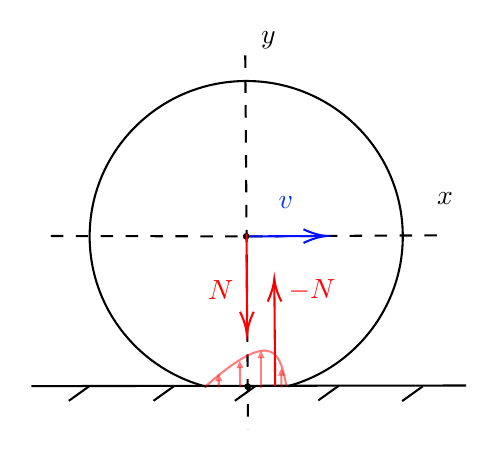
\begin{tikzpicture}[x=0.75pt,y=0.75pt,yscale=-1,xscale=1]
            %uncomment if require: \path (0,189); %set diagram left start at 0, and has height of 189

            %Straight Lines [id:da7518330174479086] 
            \draw  [dash pattern={on 4.5pt off 4.5pt}]  (6.67,90) -- (100.79,90.19) -- (193.33,89.67) ;
            %Straight Lines [id:da5592434503400421] 
            \draw	 (-2.68,162.32) -- (206.73,162.03) ;
            %Shape: Arc [id:dp1726281412706019] 
            \draw  [draw opacity=0][fill={rgb, 255:red, 8; green, 7; blue, 7 }  ,fill opacity=0 ] (81.65,162.63) .. controls (49.67,154.34) and
            (25.87,125.7) .. (25.36,91.3) .. controls (24.76,49.95) and (58.03,15.94) .. (99.69,15.33) .. controls (141.35,14.72) and (175.61,47.74) ..
            (176.22,89.08) .. controls (176.73,124) and (153.08,153.68) .. (120.62,162.44) -- (100.79,90.19) -- cycle ; \draw   (81.65,162.63) .. controls
            (49.67,154.34) and (25.87,125.7) .. (25.36,91.3) .. controls (24.76,49.95) and (58.03,15.94) .. (99.69,15.33) .. controls (141.35,14.72) and
            (175.61,47.74) .. (176.22,89.08) .. controls (176.73,124) and (153.08,153.68) .. (120.62,162.44) ;
            %Straight Lines [id:da003920177628984778] 
            \draw [color={rgb, 255:red, 4; green, 18; blue, 249 }  ,draw opacity=1 ]   (100.79,90.19) -- (137.33,90.01) ;
            \draw [shift={(139.33,90)}, rotate = 539.72] [color={rgb, 255:red, 4; green, 18; blue, 249 }  ,draw opacity=1 ][line width=0.75]
            (10.93,-3.29) .. controls (6.95,-1.4) and (3.31,-0.3) .. (0,0) .. controls (3.31,0.3) and (6.95,1.4) .. (10.93,3.29)   ;
            %Straight Lines [id:da6241641943206588] 
            \draw [color={rgb, 255:red, 0; green, 0; blue, 0 }  ,draw opacity=1 ]	(25.2,162.33) -- (15.33,169.4) ;
            %Straight Lines [id:da6421337551968986] 
            \draw [color={rgb, 255:red, 0; green, 0; blue, 0 }  ,draw opacity=1 ]	(66,162.33) -- (56.13,169.4) ;
            %Straight Lines [id:da25242184369144227] 
            \draw [color={rgb, 255:red, 0; green, 0; blue, 0 }  ,draw opacity=1 ]	(105.2,162.33) -- (95.33,169.4) ;
            %Straight Lines [id:da7965874493492349] 
            \draw [color={rgb, 255:red, 0; green, 0; blue, 0 }  ,draw opacity=1 ]	(145.4,162.13) -- (135.53,169.2) ;
            %Straight Lines [id:da2366122350933053] 
            \draw [color={rgb, 255:red, 0; green, 0; blue, 0 }  ,draw opacity=1 ]	(185.8,162.47) -- (175.93,169.53) ;
            %Straight Lines [id:da201352955590123] 
            \draw  [dash pattern={on 4.5pt off 4.5pt}]  (100.33,3) -- (101.67,183) ;
            %Straight Lines [id:da12037912623915337] 
            \draw	 (-4,15.67) ;
            %Shape: Circle [id:dp21540655765824446] 
            \draw  [color={rgb, 255:red, 0; green, 0; blue, 0 }  ,draw opacity=1 ][fill={rgb, 255:red, 0; green, 0; blue, 0 }  ,fill opacity=1 ]
            (100.45,162.53) .. controls (100.45,161.94) and (100.94,161.45) .. (101.53,161.45) .. controls (102.13,161.45) and (102.62,161.94) .. (102.62,162.53)
            .. controls (102.62,163.13) and (102.13,163.62) .. (101.53,163.62) .. controls (100.94,163.62) and (100.45,163.13) .. (100.45,162.53) -- cycle ;
            %Shape: Circle [id:dp5323977356859111] 
            \draw  [color={rgb, 255:red, 0; green, 0; blue, 0 }  ,draw opacity=1 ][fill={rgb, 255:red, 0; green, 0; blue, 0 }  ,fill opacity=1 ]
            (99.73,89.99) .. controls (99.84,89.4) and (100.4,89.01) .. (100.99,89.13) .. controls (101.58,89.24) and (101.97,89.8) .. (101.85,90.39) .. controls
            (101.74,90.98) and (101.17,91.37) .. (100.59,91.25) .. controls (100,91.14) and (99.61,90.58) .. (99.73,89.99) -- cycle ;
            %Straight Lines [id:da8962219135738276] 
            \draw [color={rgb, 255:red, 255; green, 0; blue, 0 }  ,draw opacity=1 ]   (100.99,89.13) -- (101.13,135.43) ;
            \draw [shift={(101.13,137.43)}, rotate = 269.83] [color={rgb, 255:red, 255; green, 0; blue, 0 }  ,draw opacity=1 ][line width=0.75]
            (10.93,-3.29) .. controls (6.95,-1.4) and (3.31,-0.3) .. (0,0) .. controls (3.31,0.3) and (6.95,1.4) .. (10.93,3.29)	;
            %Straight Lines [id:da7902625791767064] 
            \draw [color={rgb, 255:red, 246; green, 0; blue, 0 }  ,draw opacity=1 ][fill={rgb, 255:red, 254; green, 0; blue, 0 }  ,fill opacity=1
            ]   (114.73,162.23) -- (114.35,112.63) ;
            \draw [shift={(114.33,110.63)}, rotate = 449.56] [color={rgb, 255:red, 246; green, 0; blue, 0 }  ,draw opacity=1 ][line width=0.75]
            (10.93,-3.29) .. controls (6.95,-1.4) and (3.31,-0.3) .. (0,0) .. controls (3.31,0.3) and (6.95,1.4) .. (10.93,3.29)	;
            %Curve Lines [id:da9381909177646195] 
            \draw [color={rgb, 255:red, 255; green, 0; blue, 0 }  ,draw opacity=0.51 ]   (81.25,162.43) .. controls (115.59,132.01) and
            (117.14,148.45) .. (120.22,162.24) ;
            %Straight Lines [id:da46399317653073635] 
            \draw [color={rgb, 255:red, 255; green, 0; blue, 0 }  ,draw opacity=0.51 ]   (87.58,162.88) -- (87.55,159.32) ;
            \draw [shift={(87.53,156.32)}, rotate = 449.5] [fill={rgb, 255:red, 255; green, 0; blue, 0 }  ,fill opacity=0.51 ][line width=0.08]
            [draw opacity=0] (3.57,-1.72) -- (0,0) -- (3.57,1.72) -- cycle	  ;
            %Straight Lines [id:da977275191245905] 
            \draw [color={rgb, 255:red, 255; green, 0; blue, 0 }  ,draw opacity=0.51 ]   (97.93,162.92) -- (97.77,153.12) ;
            \draw [shift={(97.73,150.12)}, rotate = 449.1] [fill={rgb, 255:red, 255; green, 0; blue, 0 }  ,fill opacity=0.51 ][line width=0.08]
            [draw opacity=0] (3.57,-1.72) -- (0,0) -- (3.57,1.72) -- cycle	  ;
            %Straight Lines [id:da7569878460768078] 
            \draw [color={rgb, 255:red, 255; green, 0; blue, 0 }  ,draw opacity=0.51 ]   (107.93,163.12) -- (107.93,148.32) ;
            \draw [shift={(107.93,145.32)}, rotate = 450] [fill={rgb, 255:red, 255; green, 0; blue, 0 }  ,fill opacity=0.51 ][line width=0.08]
            [draw opacity=0] (3.57,-1.72) -- (0,0) -- (3.57,1.72) -- cycle	  ;
            %Straight Lines [id:da6646192752580227] 
            \draw [color={rgb, 255:red, 255; green, 0; blue, 0 }  ,draw opacity=0.51 ]   (117.78,162.93) -- (117.74,156.72) ;
            \draw [shift={(117.73,153.72)}, rotate = 449.64] [fill={rgb, 255:red, 255; green, 0; blue, 0 }	,fill opacity=0.51 ][line width=0.08]
            [draw opacity=0] (3.57,-1.72) -- (0,0) -- (3.57,1.72) -- cycle    ;

            % Text Node
            \draw (114.93,69.33) node [anchor=north west][inner sep=0.75pt]  [color={rgb, 255:red, 3; green, 49; blue, 254 }  ,opacity=1 ]
            {$v$};
            % Text Node
            \draw (80.93,109.93) node [anchor=north west][inner sep=0.75pt]  [color={rgb, 255:red, 249; green, 0; blue, 0 }  ,opacity=1 ]  {$N$};
            % Text Node
            \draw (119.73,109.53) node [anchor=north west][inner sep=0.75pt]  [color={rgb, 255:red, 247; green, 4; blue, 4 }  ,opacity=1 ]
            {$-N$};
            % Text Node
            \draw (191.33,67.53) node [anchor=north west][inner sep=0.75pt]    {$x$};
            % Text Node
            \draw (106.53,-9.87) node [anchor=north west][inner sep=0.75pt]    {$y$};

        \end{tikzpicture}
    \end{center}
    \caption*{\footnotesize Fonte: Elaborado pelo autor.}
    \label{fig:diagramaPeneu}
\end{figure}


A força de resistência ao rolamento, $F_{r}$, depende da construção do pneu e do tipo de pavimento. Essa força também depende da velocidade do
veiculo e da pressão do ar no pneu,
embora nesse trabalho não considera-se essa dependência. Para calcula-la usa-se a relação:

\begin{equation}
	\label{eq:Fr}
	F_{r}  = c_{r} \cdot N
	\enspace,
\end{equation}

em que $c_{r}$ é o coeficiente de resistência ao rolamento, $N$ é a força normal sobre o pneu e $F_{r}$ é a força
gerada pela resistência ao rolamento.
Estão apesentados na Tabela \ref{tab:ComparacaoCr}
o valor do coeficiente $c_{r}$ para pneus de uso típico em carros de passeio, bicicletas e de dois pneus específicos para a competição SEM, Michelin
45-406 e Michelin 45-75R16.

% Escrever que nao vou conciderar pq nao da pra medir a variacao no cenario atual.
% Colocar como perpestivas de trabalho futuro.

\begin{table}[H]
	\centering
	\caption{Comparação do coeficiente $c_{r}$ de diferentes pneus}
	\begin{tabular}{llll}
		\toprule
		Pneu               & $c_{r}$ &  & \\
		\hline
		Usado em carro     & 0,013   &  & \\
		Usado em bicicleta & 0,006   &  & \\
		Michelin 45-406    & 0,0024  &  & \\
		Michelin 45-75R16  & 0,00081 &  & \\
		\bottomrule
	\end{tabular}
	\caption*{\footnotesize Fonte: Adaptado de \citeauthor{book:PacCarII}.}
	\label{tab:ComparacaoCr}
\end{table}

\subsection{Sistema de propulsão}
\label{subsec:sistema_propulsao}

De forma genérica, o sistema de propulsão de um veículo elétrico, representado no diagrama da Figura \ref{fig:diagrama_propulsao}, é composto por
bateria, conversor de potencia, motor elétrico e transmissão.

\begin{figure}[H]
	\centering
	\caption{Diagrama de blocos do sistema de propulsão de um veículo elétrico}
	\label{fig:diagrama_propulsao}
	\includegraphics{DescricaoProcesso/Figuras/g874.png}
	\caption*{\footnotesize Fonte: Elaborado pelo autor.}
\end{figure}

\subsubsection{Bateria}

Bateria eletroquímica, ou apenas bateria, é um dispositivo em que durante a descarga ocorre a conversão de energia potencial química em energia
elétrica e na carga ocorre a conversão inversa. Ou seja, uma bateria armazena energia elétrica na forma de energia potencial química. Uma bateria é
composta por varais células ligadas entre se. Uma célula de bateria é basicamente composta por dois eletrodos -- positivo e
negativo -- imersos em um eletrólito\cite{book:Modern_Electric_Vehicles}.

\subsubsection{Conversor de Potência}

Conversor eletrônico de potência, ou conversor de potência, é o circuito cujo a finalidade é extrair energia elétrica de um sistema de energia e
transformá-la em uma forma adequada e necessária para um motor\cite{book:Electric_Motor_Control}.

\subsubsection{Motor Elétrico}

O motor elétrico converte a potencia elétrica -- tensão e corrente -- em potencia mecânica -- torque e rotação -- para impulsionar o
veículo\cite{book:Modern_Electric_Vehicles}. Nesse trabalho
estudara-se o modelo de apenas os motores BLDC pois é o tipo de motor utilizado no protótipo DT1.

\begin{equation}
	\label{eq:MotorCC}
	u - u_{ind}  = l_{m} \cdot \dot i + r_{m}
	\enspace,
\end{equation}

\subsubsection{Transmição}

A transmissão do veículo regula a transferência de potência do motor para as rodas. É basicamente composta por mecanismo de
redução -- ex. caixa de velocidades -- e por um mecanismo de interrupção -- ex. embreagem\cite{book:Modern_Electric_Vehicles}.

\section{Controle Ótimo}

"O objetivo da teoria de controle ótimo é determinar os sinais de controle que farão com que um processo satisfaça as restrições físicas e ao mesmo
tempo minimize
(ou maximize) alguns critérios de desempenho\cite{book:Kirk}."

A seguinte equação é uma formulação genérica e comum para OCP

\begin{mini!}
{x(\cdot),u(\cdot)}{\int_{0}^{T} L(x(t),u(t)) \,\mathrm{d}t + E(x(T)) \label{eq:ObjOCP}}
{\label{eq:formulacaoOCP}}{}
\addConstraint{x(0)-x_{0}}{=0 \label{eq:C1_OCP}}{}
\addConstraint{\dot x(t) - f(x(t),u(t))}{=0, \quad}{t \in \left[0,T\right]  \label{eq:C2_OCP}}
\addConstraint{h(x(t),u(t))}{\leq 0, \quad}{t \in \left[0,T\right]  \label{eq:C3_OCP}}
\addConstraint{r(x(T))}{\leq 0 \enspace, \label{eq:C4_OCP}}{}
\end{mini!}

em que a Equação \ref{eq:ObjOCP} é o funcional-objetivo, Equação \ref{eq:C1_OCP} é uma restrição de estados inciais fixos, Equação \ref{eq:C2_OCP} é
a restrição
que representa a dinâmica
do sistema, Equação \ref{eq:C3_OCP} são restrições de caminho e Equação \ref{eq:C4_OCP} é uma restrição de espaço para os estados finais.

O funcional-objetivo, também conhecido como objetivo de Bolza, é composto por uma integral de $L(x,u)$ conhecida como termo de Lagrange
e uma função $E(x)$ conhecida como termo de Meyer\cite{book:Numerical_Optimal_Control}.

\begin{figure}[H]
	\centering
	\caption{Visão geral do métodos numéricos para controle ótimo}
	\label{fig:diagrama_metodos_numericos}
	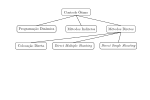
\includegraphics{DescricaoProcesso/Figuras/diagrama_metodos_numericos.png}
	\caption*{\footnotesize Fonte: Adaptado de \citeauthor{article:Diehl}}
\end{figure}

\cite{phd:Matthias} \cite{phd:Rieck} \cite{manual:Falcon}

\clearpage